\documentclass[11pt]{article}
\usepackage[margin=1in]{geometry}
\usepackage{amsmath,amssymb,bm}
\usepackage{booktabs}
\usepackage{graphicx}
\usepackage{float}
\usepackage{caption}
\usepackage{hyperref}
\usepackage{array}
\captionsetup{font=small,labelfont=bf}
\graphicspath{{outputs/figures/}}

\newcommand{\Normal}{\mathcal{N}}
\newcommand{\Prob}{\mathbb{P}}
\newcommand{\Ind}{\mathbb{I}}

\title{A Bayesian Hierarchical Threshold-Crossing Model for Irregular\\
Molecular Monitoring: Specification and Fitted Results}
\author{}
\date{\today}

\begin{document}
\maketitle

\begin{abstract}
\noindent This report documents the primary model --- a Bayesian multi-state latent
threshold-crossing joint model with a flexible (linear-spline) trajectory ---
for irregular molecular monitoring in chronic myeloid leukemia (CML), and its
fit to the real cohort by Hamiltonian Monte Carlo in Stan. A single-state
threshold model and an interval-hazard comparator, fitted to a simulated cohort,
form a development and recovery study. The model
couples a latent patient-specific log-MRD trajectory, assay-floor
left-censoring, and a latent threshold-crossing definition of deep molecular
response (DMR) observed only at irregular visits. Estimation, posterior
predictive checks, calibration, and dynamic prediction are reported. The primary result is the multi-state spline fit to the $N=87$ CML cohort
(Section~\ref{sec:spline-real}); the recovery study uses a simulated $N=200$
cohort generated from the fitted-model parameters.
\end{abstract}

\section{Model}

\subsection{Latent trajectory and assay model}
Let $i=1,\dots,N$ index patients and $j=1,\dots,n_i$ monitoring visits at
times $t_{ij}$ (years). With $\ell(t)=\log(1+t)$, the latent log-MRD
trajectory is
\begin{equation}
m_i(t)=\beta_0+\beta_1\ell(t)+\beta_2\ell(t)^2+b_{0i}+b_{1i}\ell(t),
\qquad b_{0i}\sim\Normal(0,\tau_0^2),\; b_{1i}\sim\Normal(0,\tau_1^2),
\end{equation}
with independent random effects. The observation-scale mean adds a
sample-source term, $\mu_{ij}=m_i(t_{ij})+\beta_{\mathrm{BM}}\,
\Ind(s_{ij}=\text{bone marrow})$. Writing the assay floor $c_F=-5.0$, a
non-floor measurement contributes $\tfrac{1}{\sigma_y}\phi\!\big((y_{ij}-
\mu_{ij})/\sigma_y\big)$ and a floor measurement is \emph{left-censored},
contributing $\Phi\!\big((c_F-\mu_{ij})/\sigma_y\big)$.

\subsection{Latent threshold-crossing DMR}
DMR is defined through the biomarker itself, $c_D=-4.5$, so DMR onset is the
first crossing $T_i^{D}=\inf\{t\ge0:m_i(t)\le c_D\}$. With the running minimum
$M_i(t)=\min_{0\le u\le t}m_i(u)$ one has $T_i^{D}\le t\Leftrightarrow
M_i(t)\le c_D$. Because response is documented only at visits, DMR is
interval-observed. Introducing threshold uncertainty $C_i^{D}\sim
\Normal(c_D,\sigma_{\mathrm{thr}}^2)$, an observed DMR interval $(L_i,R_i]$
contributes
\begin{equation}
\Phi\!\Big(\tfrac{M_i(L_i)-c_D}{\sigma_{\mathrm{thr}}}\Big)
-\Phi\!\Big(\tfrac{M_i(R_i)-c_D}{\sigma_{\mathrm{thr}}}\Big),
\end{equation}
and a censored patient contributes $\Phi\!\big((M_i(C_i)-c_D)/
\sigma_{\mathrm{thr}}\big)$. For HMC the running minimum is approximated by a
differentiable soft-min over a grid $0=u_1<\dots<u_G=t$,
$M_i^{(\kappa)}(t)=-\kappa^{-1}\log\sum_{g}\exp\{-\kappa\, m_i(u_g)\}$, and the
CDF difference is evaluated with a stable log-difference. This soft-min
single-state model is a \emph{development version}: the analytic
piecewise-quadratic multi-state model with a spline trajectory
(Section~\ref{sec:spline-real}) supersedes it, computing the running minimum and
maximum in closed form and sampling without divergences.

\subsection{Interval-hazard comparator}
For comparison, first \emph{documented} DMR in at-risk interval $k$
(length $\Delta_{ik}$, midpoint $t^{mid}_{ik}$) uses a complementary log-log
hazard $h^{D}_{ik}=\exp\{\gamma_0+\gamma_1\log(1+t^{mid}_{ik})+\gamma_2
\log(1+\Delta_{ik})+\alpha\,m_i(t^{mid}_{ik})\}$ with interval event
probability $p^{D}_{ik}=1-\exp(-h^{D}_{ik}\Delta_{ik})$.

\subsection{Priors}
$\beta_0\sim\Normal(-2.5,2^2)$, $\beta_1\sim\Normal(-1,1^2)$,
$\beta_2\sim\Normal(0,0.5^2)$, $\beta_{\mathrm{BM}}\sim\Normal(0,1^2)$,
$\sigma_y,\tau_0,\tau_1\sim\mathrm{Exp}(1)$,
$\sigma_{\mathrm{thr}}\sim\text{Half-}\Normal(0,0.25^2)$; and for the
comparator $\gamma_0\sim\Normal(-2,2^2)$, $\gamma_1,\gamma_2\sim\Normal(0,1^2)$,
$\alpha\sim\Normal(-0.5,0.75^2)$.

\section{Estimation}
Both models were fit by HMC in Stan (\texttt{cmdstanr}) with 4 chains,
$1000$ warmup $+1000$ sampling iterations each, non-centred random effects,
soft-min grid $G=60$ and sharpness $\kappa=50$, and model-appropriate initial
values (random starts make the threshold likelihood evaluate to $\log 0$).
Data were simulated from the parameters in the ``Truth'' columns of
Tables~\ref{tab:post-thr}--\ref{tab:post-int} ($N=200$, non-informative
monitoring), enabling assessment of parameter recovery.

\section{Primary result: multi-state spline model fitted to the CML cohort}
\label{sec:spline-real}

The primary model is the multi-state latent threshold-crossing joint model with
a flexible (linear-spline) trajectory (Stan file \texttt{multistate\_spline.stan}).
We fitted the bidirectional multi-state model with the linear-spline (hinge)
trajectory --- a patient-specific slope change $\zeta_i\sim N(0,\sigma_\zeta^2)$
after a two-year knot --- to the real CML cohort ($N=87$; 68 DMR onsets, 9
confirmed molecular relapses) by Hamiltonian Monte Carlo (4 chains,
$2000+2000$ iterations, \texttt{adapt\_delta}$=0.999$). Because the trajectory
is piecewise-quadratic the running minimum and post-knot values are closed form,
so no soft-min grid is needed. Sampling was clean: all $\widehat R\le1.002$ and
bulk effective sample size exceeded $2000$ for every parameter
(Table~\ref{tab:spline-real}). The patient-specific post-knot slope
$\sigma_\zeta=6.43$ (90\% interval $5.01$--$7.97$) is strongly identified,
confirming that individual late rebounds --- and hence molecular relapse --- are
a real feature that the flexible trajectory captures; this resolves the relapse
under-prediction of the convex-quadratic model (relapse Brier $0.082\to0.054$ in
the marginal-likelihood validation). With the spline explaining the crossings,
the threshold width is near zero ($\sigma_{\mathrm{thr}}=0.06$). The longitudinal
parameters reproduce the single-state and base multi-state fits.

\begin{table}[H]
\centering
\caption{Multi-state spline model fitted to the CML cohort ($N=87$) by HMC. Posterior mean, $90\%$ credible interval, $\widehat R$ and bulk effective sample size (ESS).}
\label{tab:spline-real}
\begin{tabular}{lrrrr}
\toprule
Parameter & Mean & $90\%$ interval & $\widehat R$ & ESS\\
\midrule
$\beta_0$                & $-2.02$ & $(-2.36,-1.65)$ & 1.000 & 4568\\
$\beta_{\mathrm{time}}$  & $-4.03$ & $(-4.76,-3.33)$ & 1.000 & 4454\\
$\beta_{\mathrm{time}^2}$& $0.94$  & $(0.55,1.36)$   & 1.000 & 5058\\
$\beta_{\mathrm{BM}}$    & $0.69$  & $(0.49,0.88)$   & 1.001 & 9129\\
$\sigma_y$               & $1.62$  & $(1.48,1.76)$   & 1.001 & 10455\\
$\tau_{b0}$              & $1.07$  & $(0.86,1.31)$   & 1.002 & 3152\\
$\tau_{b1}$              & $2.33$  & $(1.83,2.90)$   & 1.002 & 2580\\
$\sigma_\zeta$           & $6.43$  & $(5.01,7.97)$   & 1.001 & 4885\\
$\sigma_{\mathrm{thr}}$  & $0.06$  & $(0.02,0.13)$   & 1.000 & 2255\\
\bottomrule
\end{tabular}
\end{table}

\begin{figure}[H]
\centering
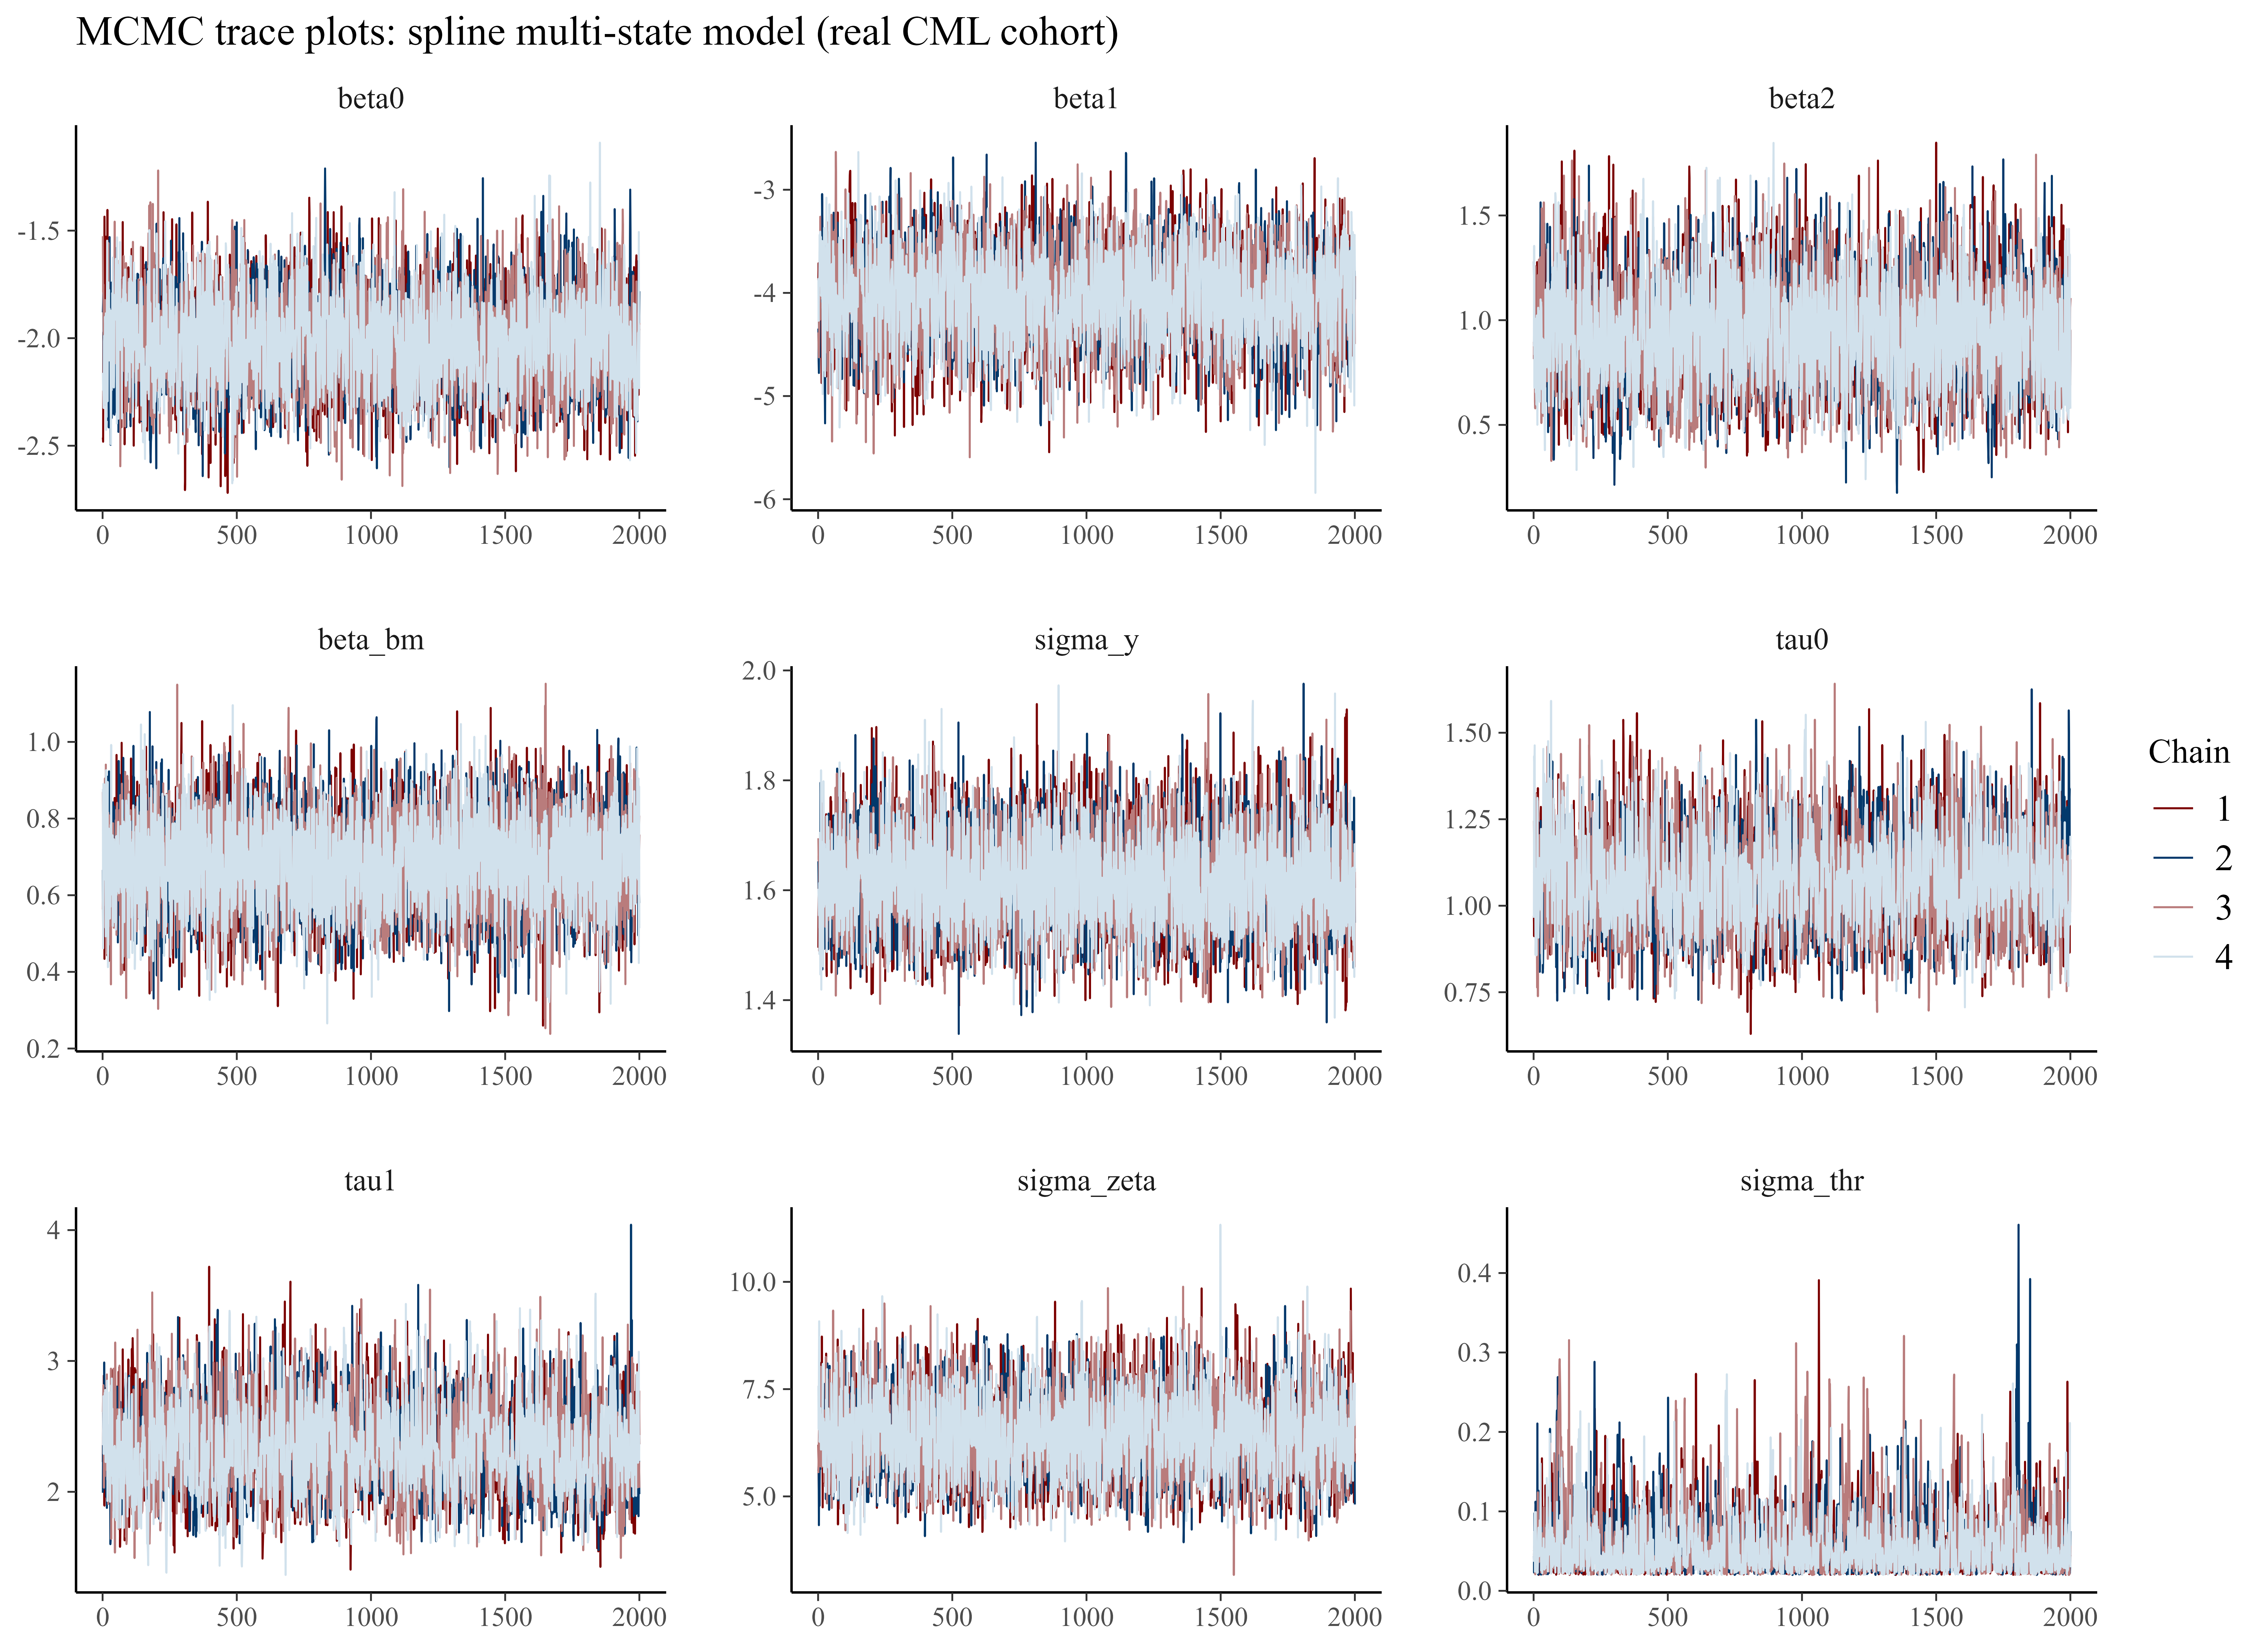
\includegraphics[width=0.95\linewidth]{figR_18_trace_spline.png}
\caption{Hamiltonian Monte Carlo trace plots for the spline multi-state model fitted to the CML cohort (4 chains, 2000 post-warmup iterations each). All parameters mix well, with stationary, fully overlapping chains and no drift or stuck segments, consistent with $\widehat R\le1.002$ and bulk effective sample size $>2000$ (Table~\ref{tab:spline-real}). The threshold width $\sigma_{\mathrm{thr}}$ sits near its lower bound, reflecting that the flexible trajectory renders the crossings nearly deterministic.}
\label{fig:trace-spline}
\end{figure}

\section{Development and recovery study (simulated cohort)}

The results below validate the shared longitudinal and assay-floor components,
and the interval-hazard comparator, on a simulated demonstration cohort
($N=200$) with known data-generating truth. The soft-min single-state threshold
model here is a development version superseded by the multi-state spline model of
Section~\ref{sec:spline-real}.

\subsection{Posterior summaries}
Tables~\ref{tab:post-thr} and \ref{tab:post-int} report posterior means, 90\%
intervals, and convergence diagnostics for the two models. The longitudinal
structure is recovered well by both; the threshold model estimates a larger
effective threshold width $\sigma_{\mathrm{thr}}$ than the data-generating
value because documentation depends on the \emph{measured} (noisy) biomarker
rather than the latent crossing.

\begin{table}[H]
\centering
\caption{Threshold-crossing model: posterior summaries ($N=200$ simulated cohort).}
\label{tab:post-thr}
\begin{tabular}{lrrrrrr}
\toprule
Parameter & Mean & 5\% & 95\% & $\widehat R$ & ESS$_{\mathrm{bulk}}$ & Truth\\
\midrule
$\beta_0$              & $-2.00$ & $-2.25$ & $-1.76$ & 1.001 & 3249 & $-2.074$\\
$\beta_{\mathrm{time}}$& $-3.56$ & $-4.04$ & $-3.09$ & 1.001 & 2636 & $-3.561$\\
$\beta_{\mathrm{time}^2}$& $0.60$ & $0.35$ & $0.84$ & 1.001 & 3273 & $0.502$\\
$\beta_{\mathrm{BM}}$  & $0.76$ & $0.61$ & $0.90$ & 1.001 & 4948 & $0.607$\\
$\sigma_y$             & $1.71$ & $1.64$ & $1.80$ & 1.001 & 4159 & $1.813$\\
$\tau_{b0}$            & $1.20$ & $1.03$ & $1.38$ & 1.007 & 1348 & $0.968$\\
$\tau_{b1}$            & $2.09$ & $1.84$ & $2.36$ & 1.004 & 1790 & $2.203$\\
$\sigma_{\mathrm{thr}}$& $0.61$ & $0.47$ & $0.75$ & 1.004 & 1446 & $0.200$\\
\bottomrule
\end{tabular}
\end{table}

\begin{table}[H]
\centering
\caption{Interval-hazard comparator: posterior summaries ($N=200$ simulated cohort).}
\label{tab:post-int}
\begin{tabular}{lrrrrrr}
\toprule
Parameter & Mean & 5\% & 95\% & $\widehat R$ & ESS$_{\mathrm{bulk}}$ & Truth\\
\midrule
$\beta_0$              & $-2.11$ & $-2.49$ & $-1.74$ & 1.000 & 6223 & $-2.074$\\
$\beta_{\mathrm{time}}$& $-3.23$ & $-3.75$ & $-2.72$ & 1.001 & 4646 & $-3.561$\\
$\beta_{\mathrm{time}^2}$& $0.45$ & $0.19$ & $0.73$ & 1.000 & 6376 & $0.502$\\
$\beta_{\mathrm{BM}}$  & $0.68$ & $0.36$ & $1.01$ & 1.000 & 7236 & $0.607$\\
$\sigma_y$             & $1.69$ & $1.62$ & $1.77$ & 1.000 & 5215 & $1.813$\\
$\tau_{b0}$            & $1.37$ & $1.19$ & $1.56$ & 1.000 & 2241 & $0.968$\\
$\tau_{b1}$            & $2.22$ & $1.95$ & $2.51$ & 1.002 & 2106 & $2.203$\\
$\gamma_0$             & $-5.68$ & $-7.23$ & $-4.31$ & 1.001 & 3172 & $-4.095$\\
$\gamma_{\mathrm{time}}$& $-0.68$ & $-1.29$ & $-0.08$ & 1.000 & 7934 & $-0.228$\\
$\gamma_{\mathrm{gap}}$& $-2.32$ & $-3.17$ & $-1.50$ & 1.001 & 7555 & $-1.831$\\
$\alpha_{\mathrm{MRD}}$& $-1.77$ & $-2.15$ & $-1.45$ & 1.001 & 3161 & $-1.275$\\
\bottomrule
\end{tabular}
\end{table}

\subsection{Sampler diagnostics}
Table~\ref{tab:diag} summarizes HMC diagnostics. The interval-hazard model
sampled cleanly. The threshold-crossing model converged in $\widehat R$ and
effective sample size but produced $219$ divergent transitions out of $4000$
post-warmup draws, indicating a challenging posterior geometry induced by the
soft-min running-minimum term. For confirmatory analyses this should be
mitigated by raising \texttt{adapt\_delta} (e.g.\ to $0.99$), increasing the
soft-min sharpness grid, or reparameterizing the threshold term; the
divergences are reported here transparently rather than suppressed.

\begin{table}[H]
\centering
\caption{Hamiltonian Monte Carlo diagnostics (4 chains, 4000 post-warmup draws).}
\label{tab:diag}
\begin{tabular}{lrrrrr}
\toprule
Model & Divergences & Max treedepth hits & Min E-BFMI & Max $\widehat R$ & Min ESS$_{\mathrm{bulk}}$\\
\midrule
Threshold-crossing & 219 & 0 & 0.519 & 1.007 & 1348\\
Interval-hazard    & 0   & 0 & 0.566 & 1.002 & 2106\\
\bottomrule
\end{tabular}
\end{table}

\subsection{Posterior predictive checks and calibration}
The longitudinal assay model is well calibrated: the observed assay-floor rate
was $0.408$ versus a posterior mean floor probability of $0.407$, and non-floor
predictive interval coverage was $0.950$ ($90\%$) and $0.976$ ($95\%$).
Patient-level DMR calibration for the threshold model gave a Brier score of
$0.016$, with mean predicted DMR probability $0.73$ against an observed rate of
$0.76$; the calibration slope of $2.70$ indicates the raw mechanistic
probabilities are under-dispersed and benefit from recalibration.
Figures~\ref{fig:traj}--\ref{fig:cal} display the trajectories, the
assay-floor posterior predictive check, and the grouped DMR calibration.

\begin{figure}[H]
\centering
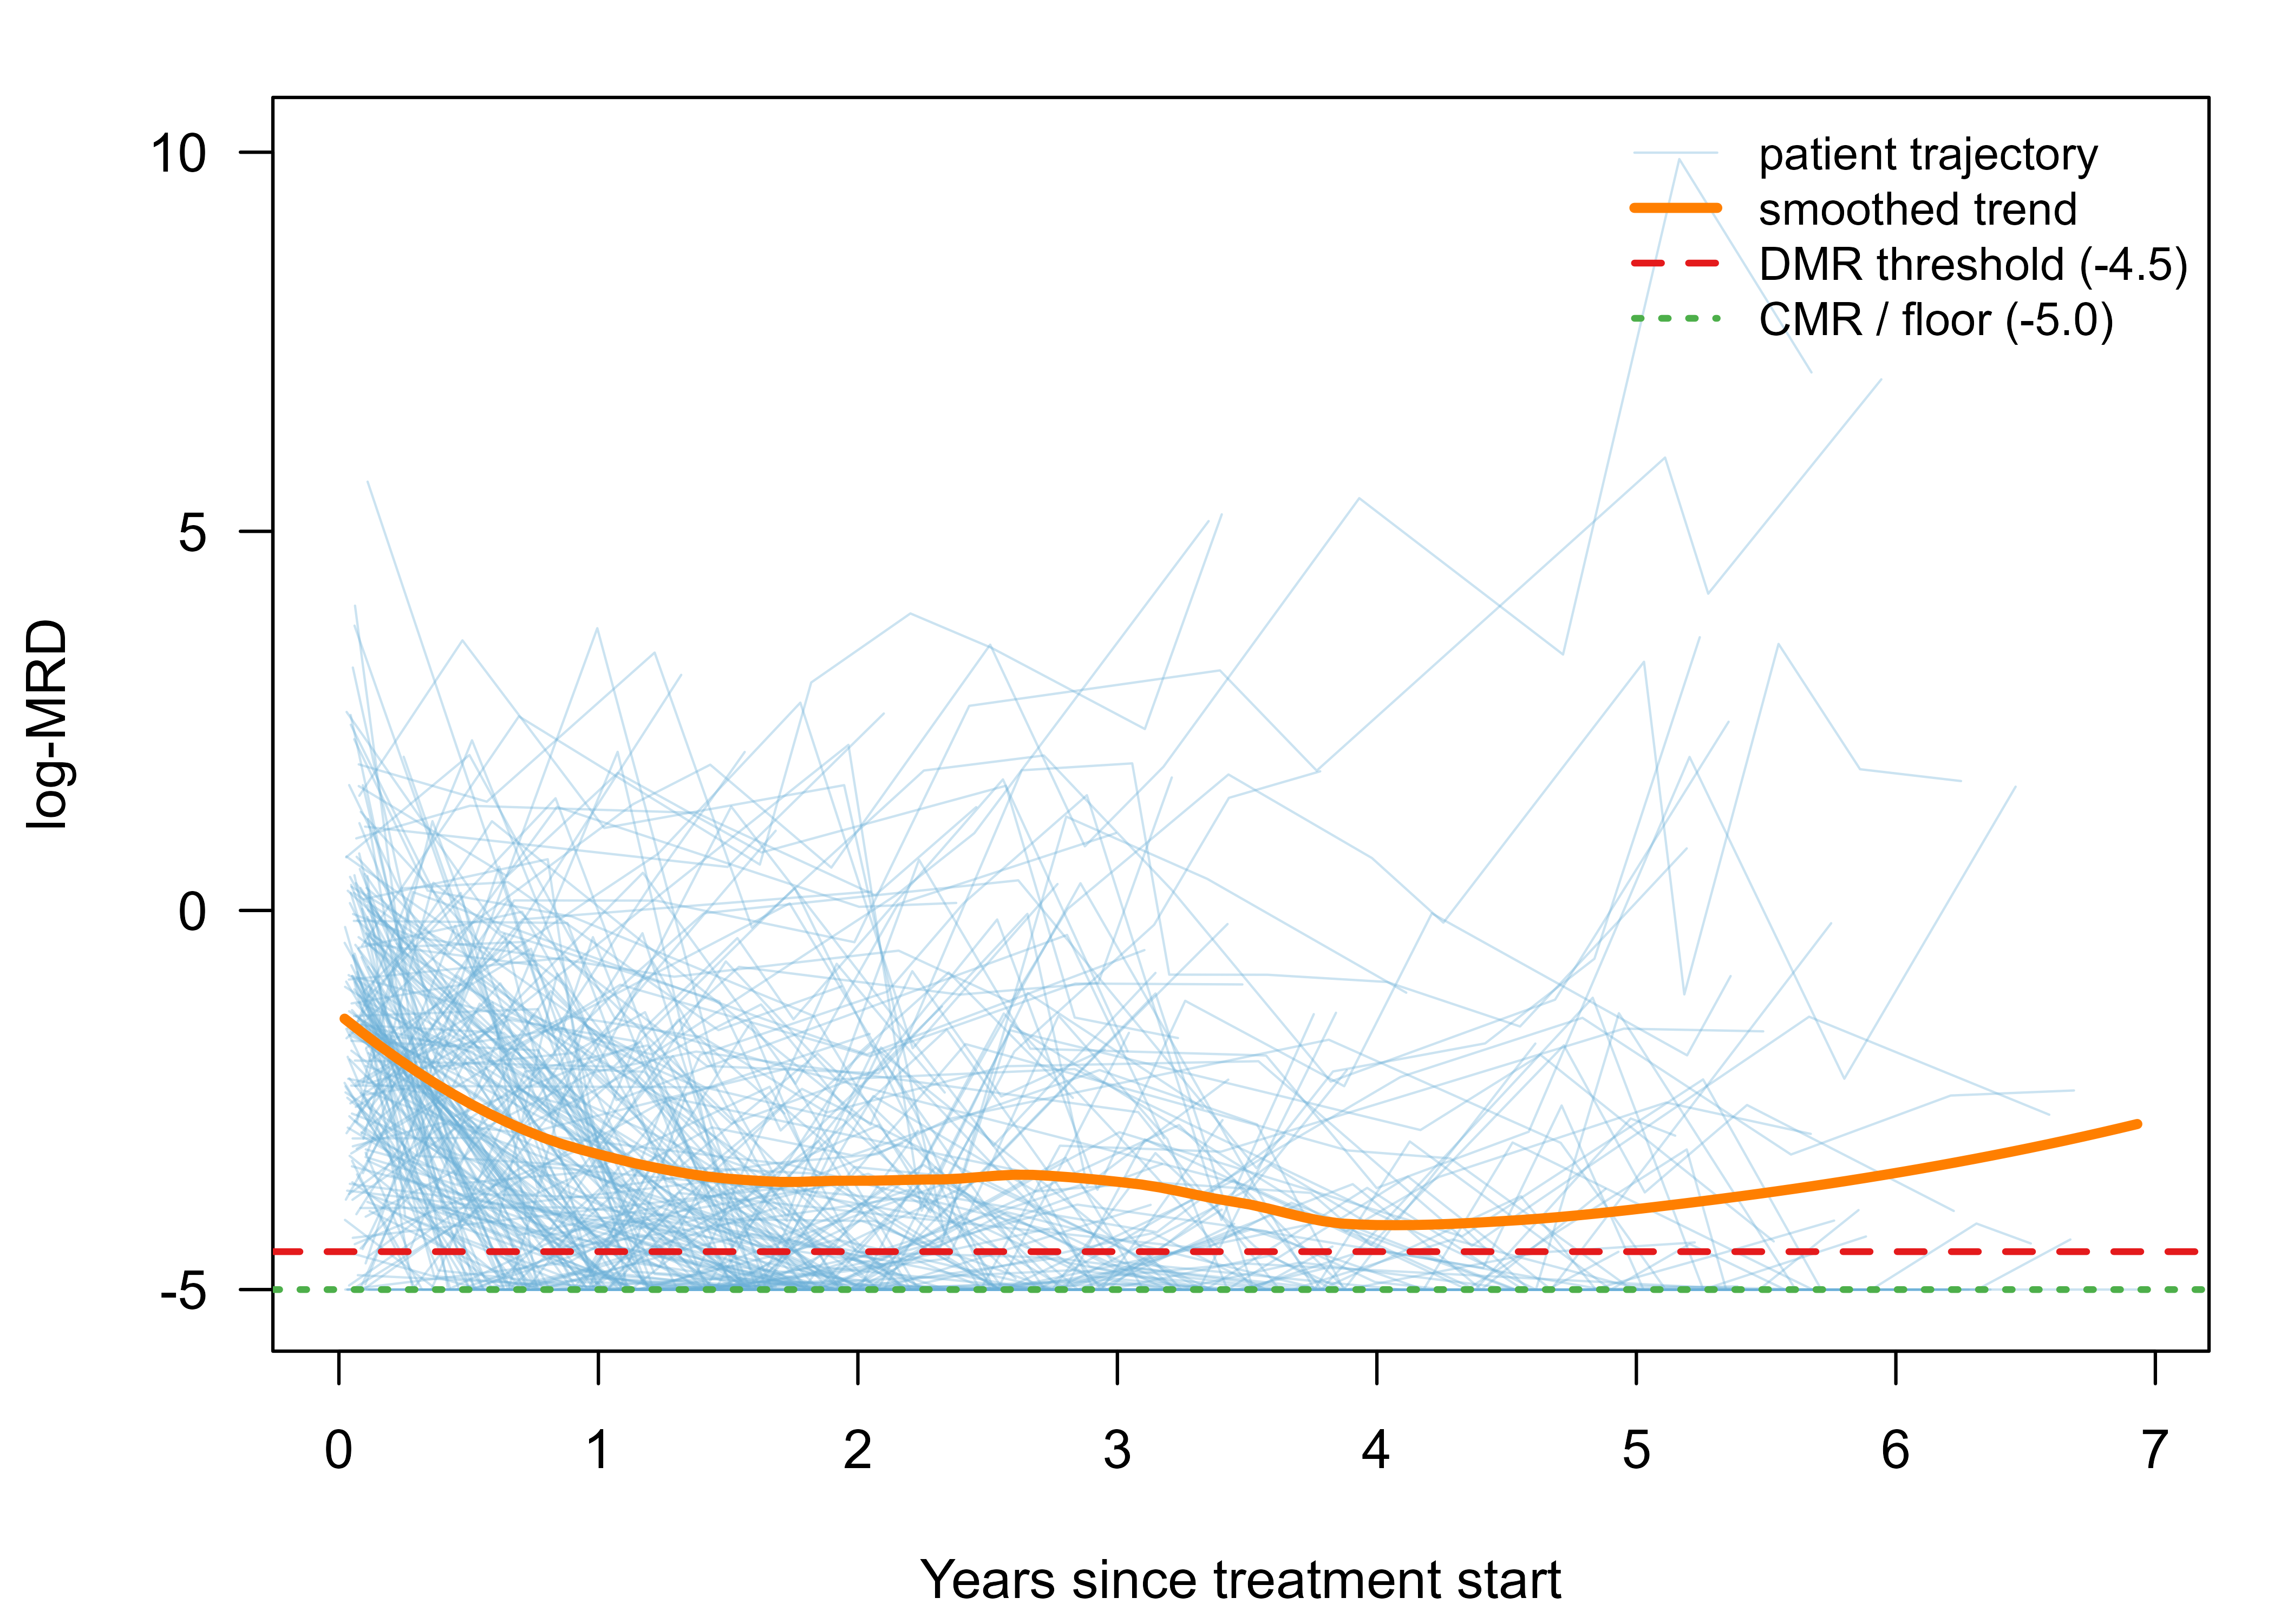
\includegraphics[width=0.8\linewidth]{figR_01_trajectories.png}
\caption{Simulated patient-level log-MRD trajectories with smoothed population
trend and the DMR ($-4.5$) and floor ($-5.0$) thresholds.}
\label{fig:traj}
\end{figure}

\begin{figure}[H]
\centering
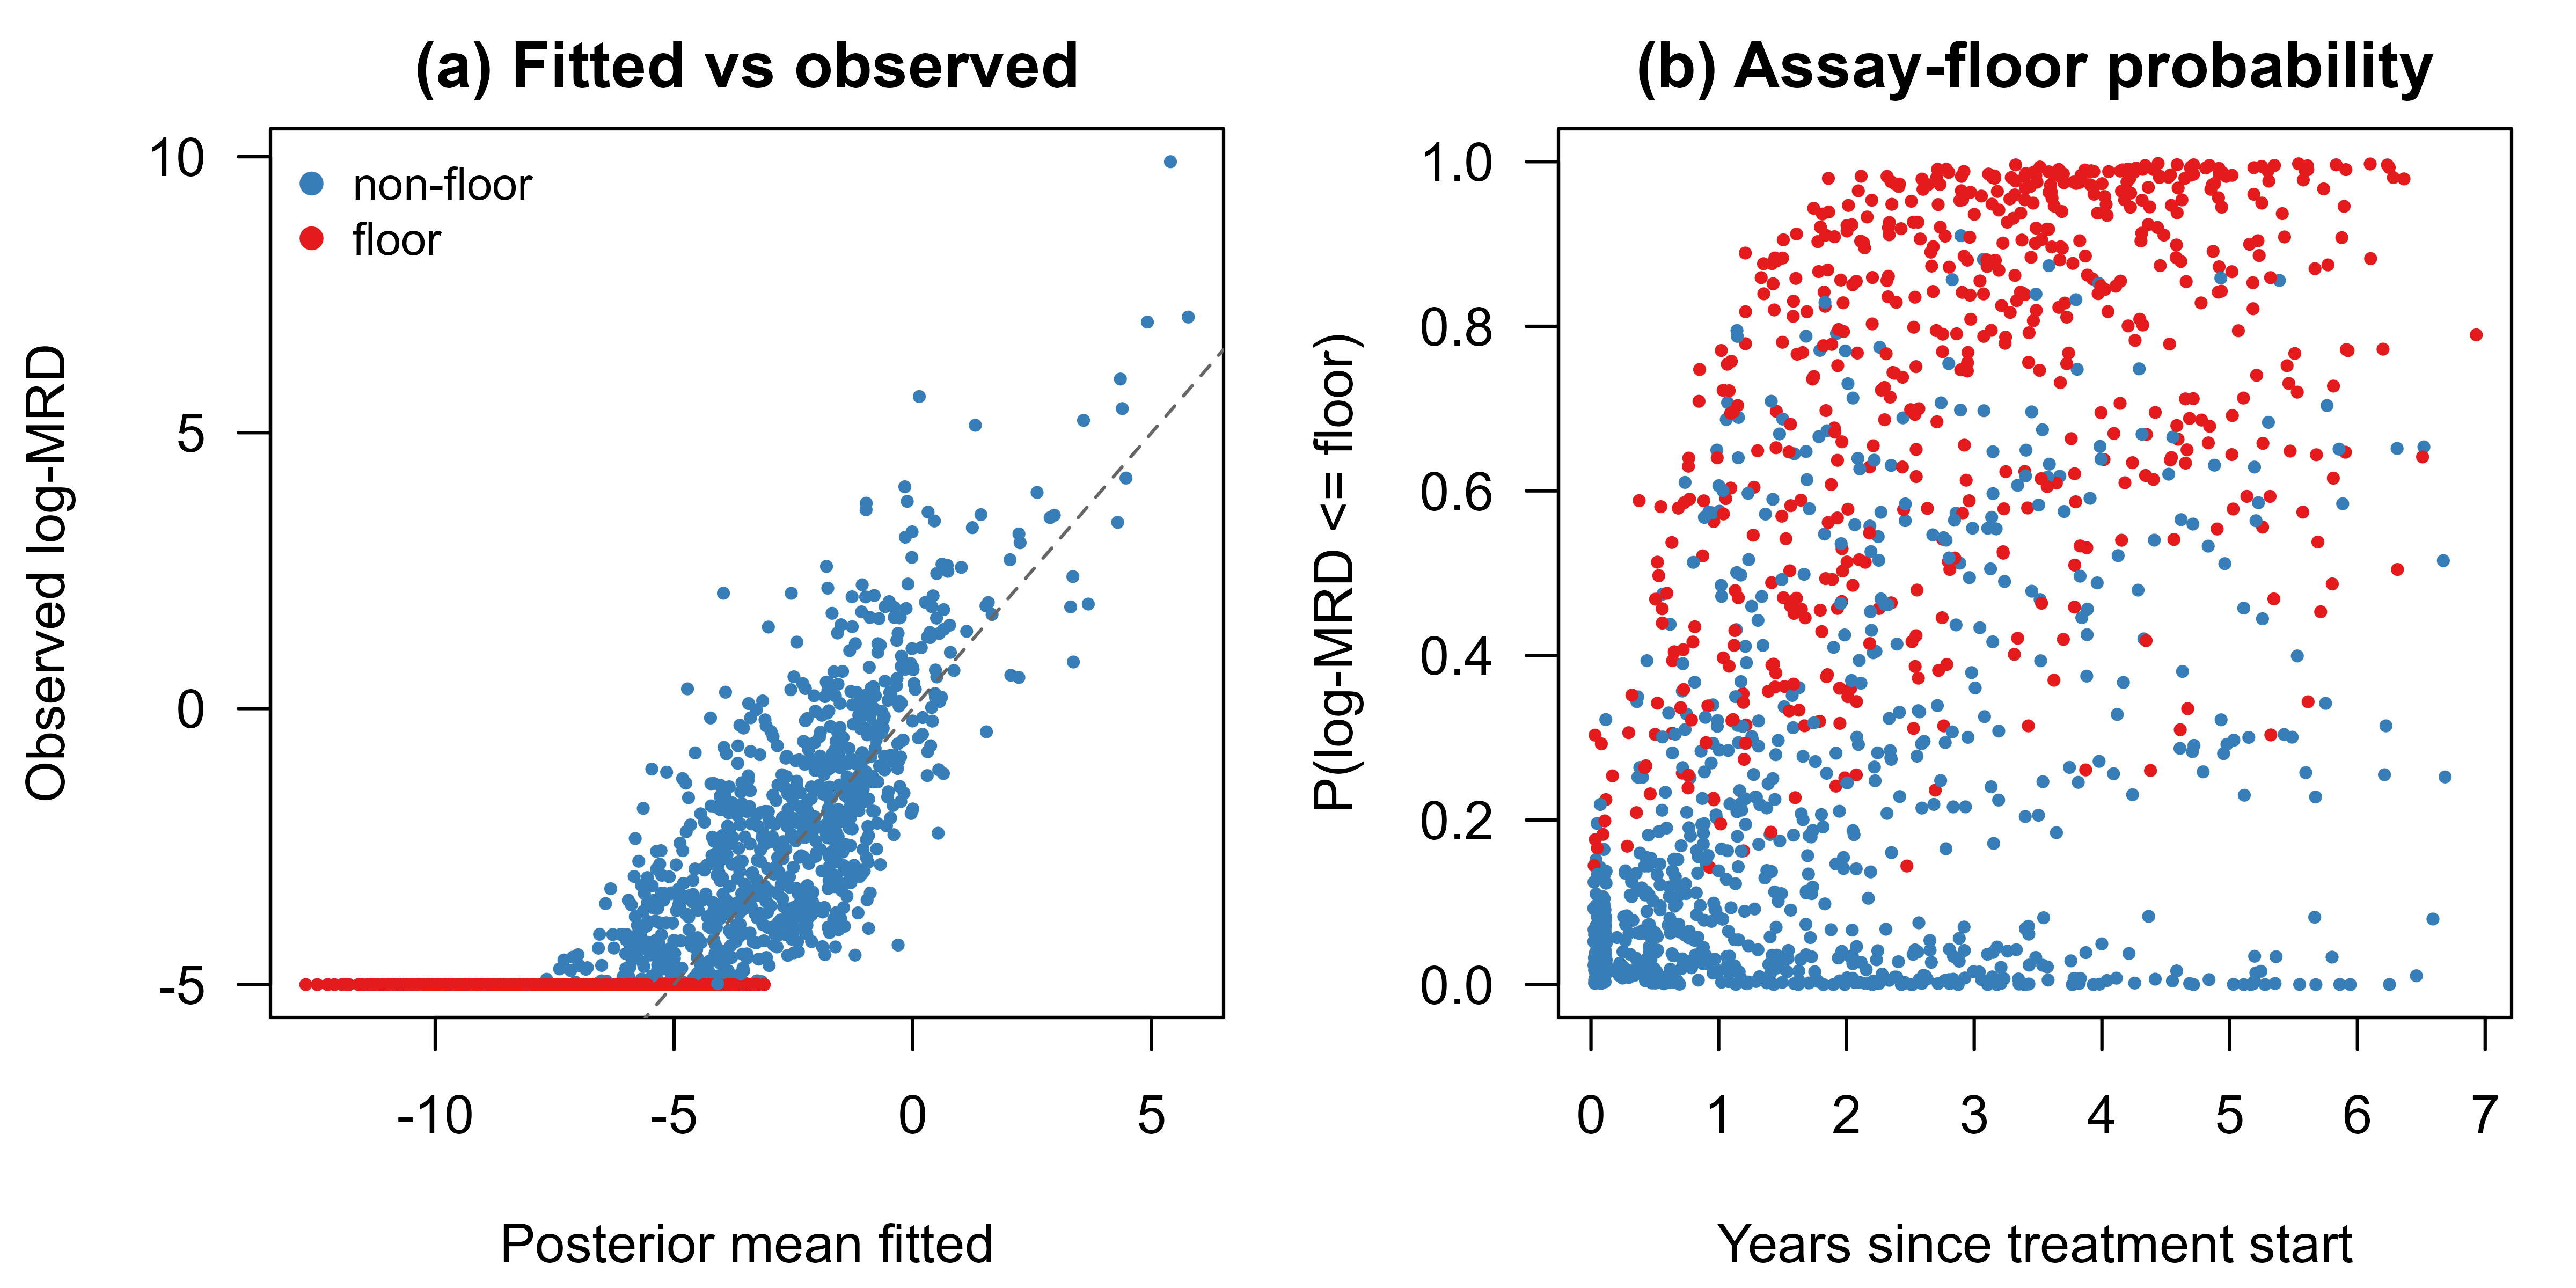
\includegraphics[width=0.95\linewidth]{figR_02_ppc_floor.png}
\caption{Assay-floor posterior predictive check: (a) posterior-mean fitted vs
observed log-MRD; (b) posterior probability of a floor observation over time,
distinguishing observed floor and non-floor measurements.}
\label{fig:ppc}
\end{figure}

\begin{figure}[H]
\centering
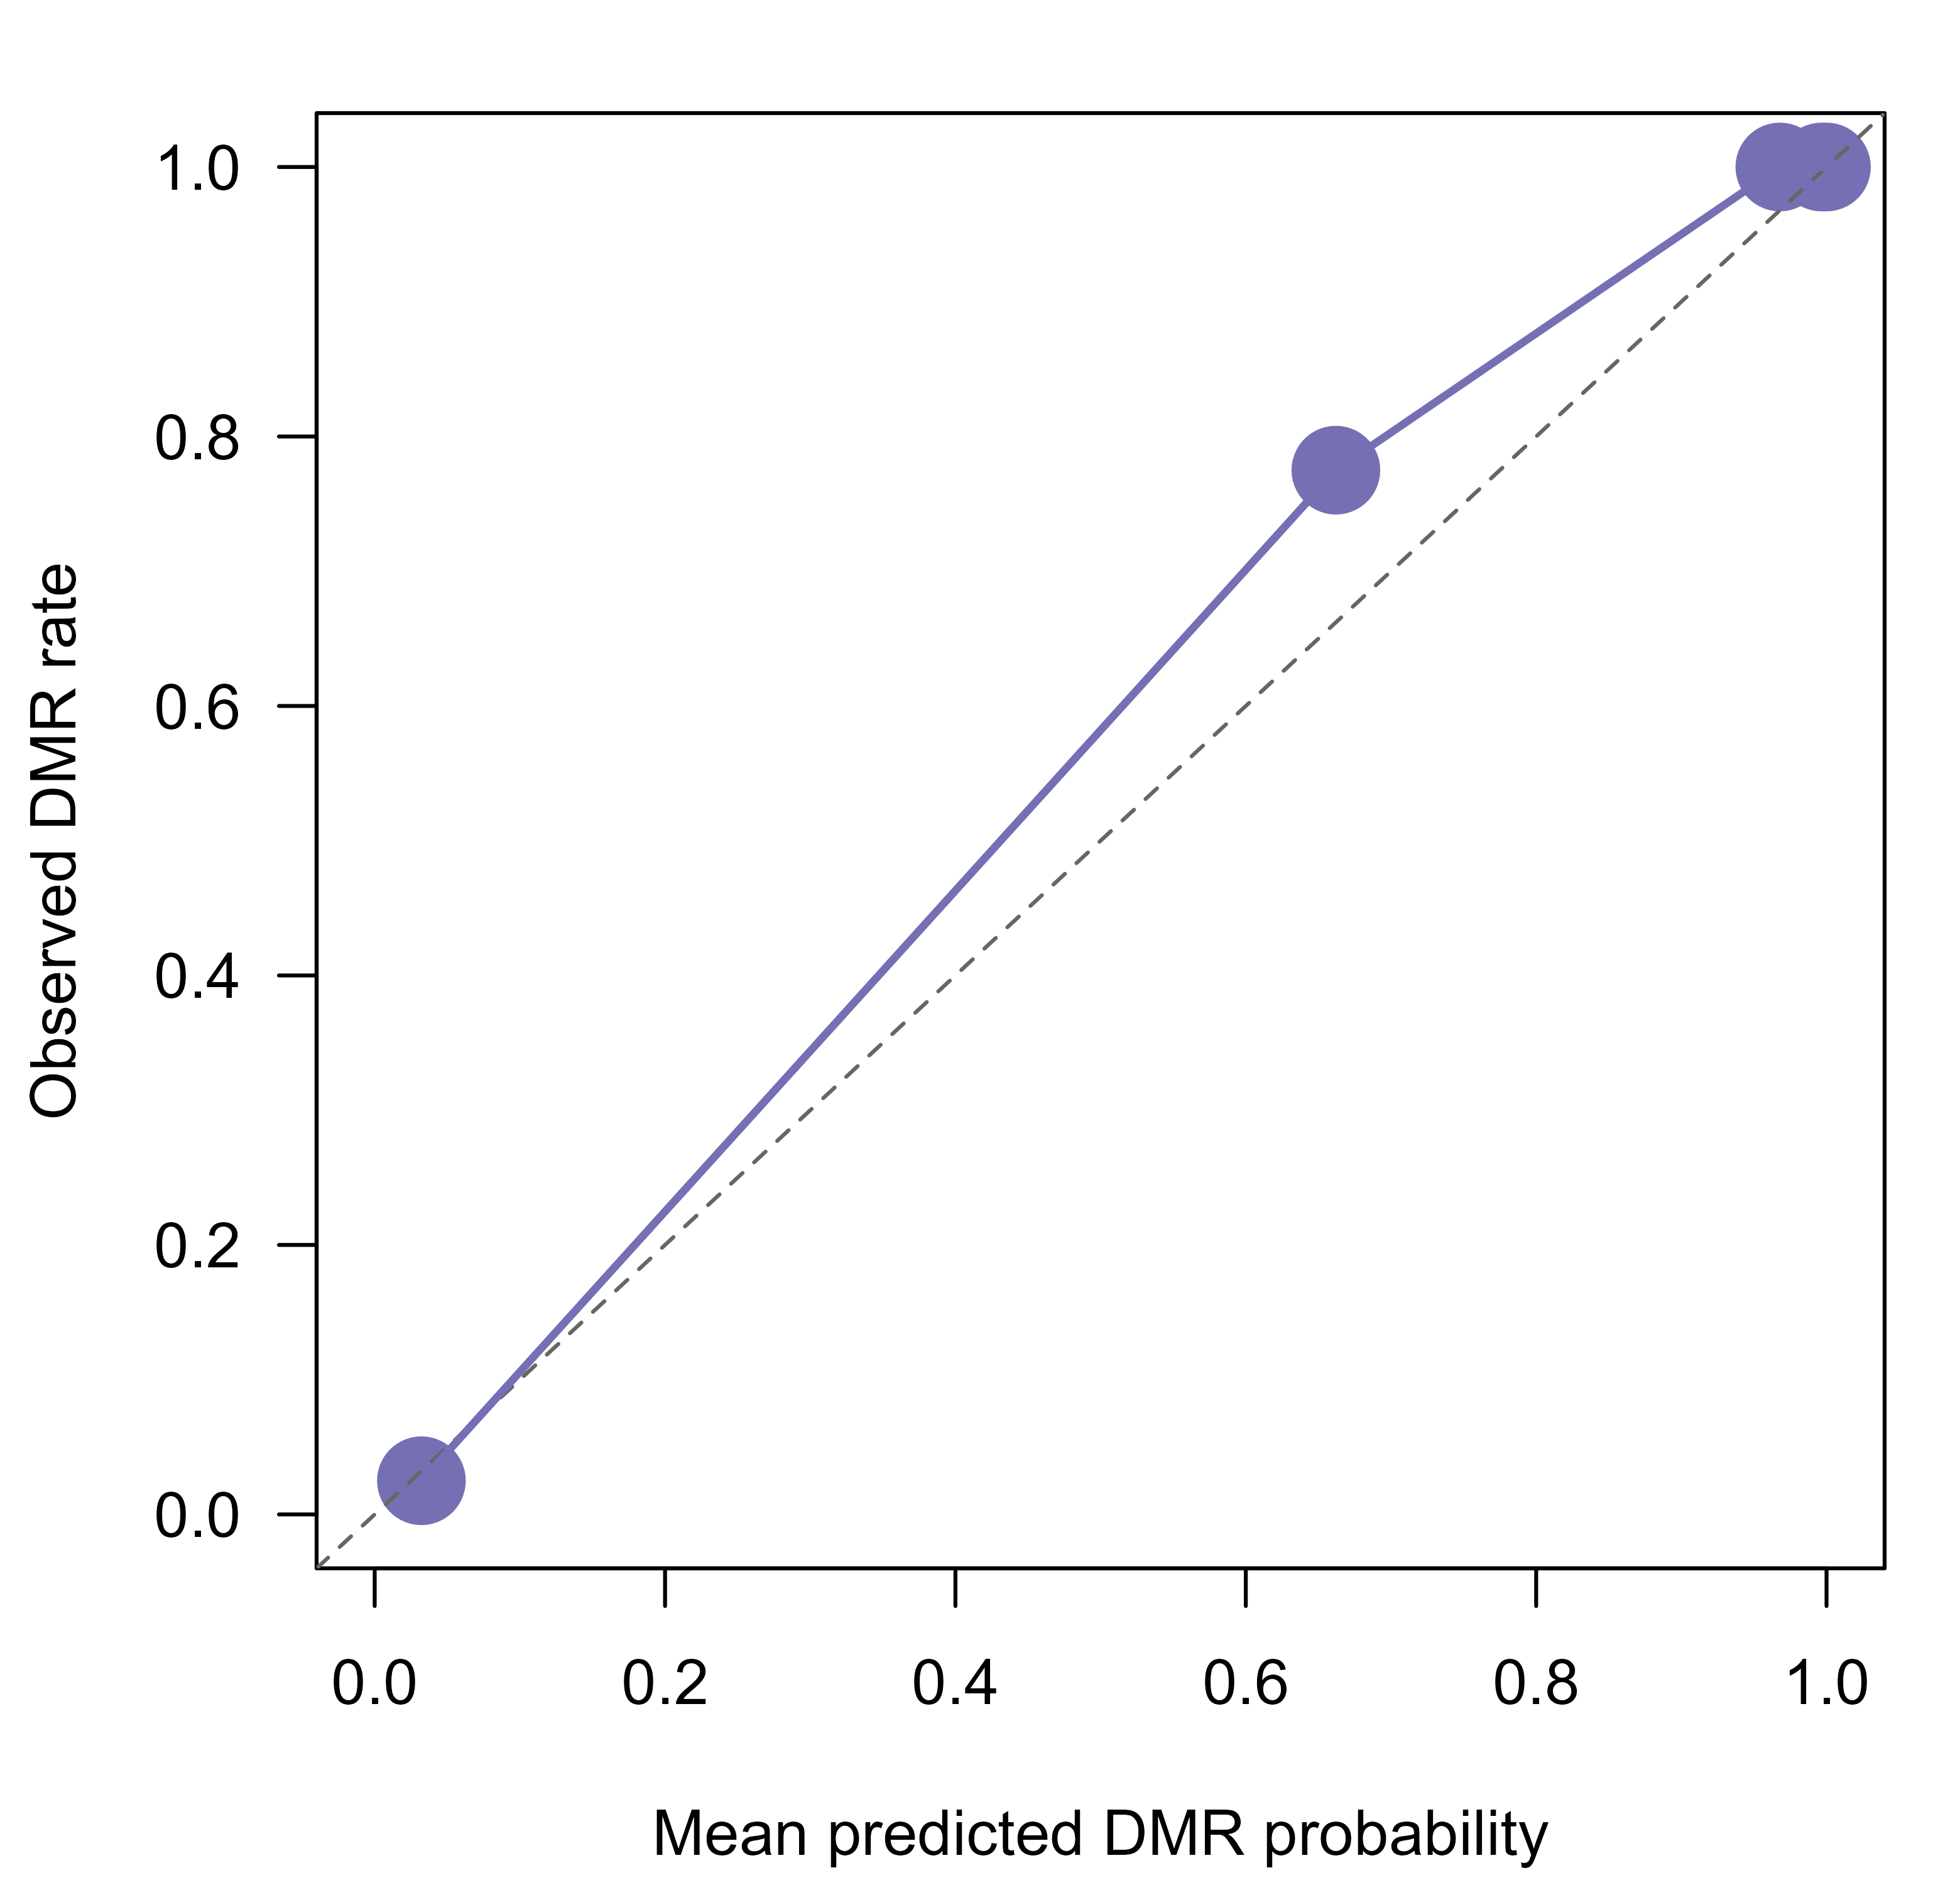
\includegraphics[width=0.55\linewidth]{figR_03_dmr_calibration.png}
\caption{Grouped calibration of predicted patient-level DMR probability against
the observed DMR rate (point size proportional to bin count).}
\label{fig:cal}
\end{figure}

\subsection{Dynamic prediction}
Table~\ref{tab:dyn} and Figure~\ref{fig:dyn} report landmark dynamic
predictions $\pi_i(s,H)=\Prob(T_i^{D}\le s+H\mid T_i^{D}>s,\mathcal H_i(s))$.
Predicted and observed within-horizon DMR probabilities agree closely at early
landmarks and short horizons and show the expected over-prediction at later
landmarks/longer horizons that motivates horizon-specific recalibration.

\begin{table}[H]
\centering
\caption{Landmark dynamic prediction of DMR by horizon $H$ (years).}
\label{tab:dyn}
\begin{tabular}{rrrrrr}
\toprule
Landmark $s$ & Horizon $H$ & At risk & Mean predicted & Observed & Brier\\
\midrule
0.5 & 0.5 & 159 & 0.330 & 0.314 & 0.139\\
0.5 & 1.0 & 159 & 0.497 & 0.465 & 0.125\\
0.5 & 2.0 & 159 & 0.625 & 0.560 & 0.137\\
1.0 & 0.5 & 109 & 0.270 & 0.220 & 0.134\\
1.0 & 1.0 & 109 & 0.388 & 0.312 & 0.176\\
1.0 & 2.0 & 109 & 0.488 & 0.404 & 0.192\\
1.5 & 0.5 &  85 & 0.215 & 0.118 & 0.139\\
1.5 & 1.0 &  85 & 0.313 & 0.176 & 0.186\\
1.5 & 2.0 &  85 & 0.397 & 0.271 & 0.200\\
2.0 & 0.5 &  75 & 0.196 & 0.067 & 0.127\\
2.0 & 1.0 &  75 & 0.274 & 0.133 & 0.188\\
2.0 & 2.0 &  75 & 0.341 & 0.187 & 0.231\\
\bottomrule
\end{tabular}
\end{table}

\begin{figure}[H]
\centering
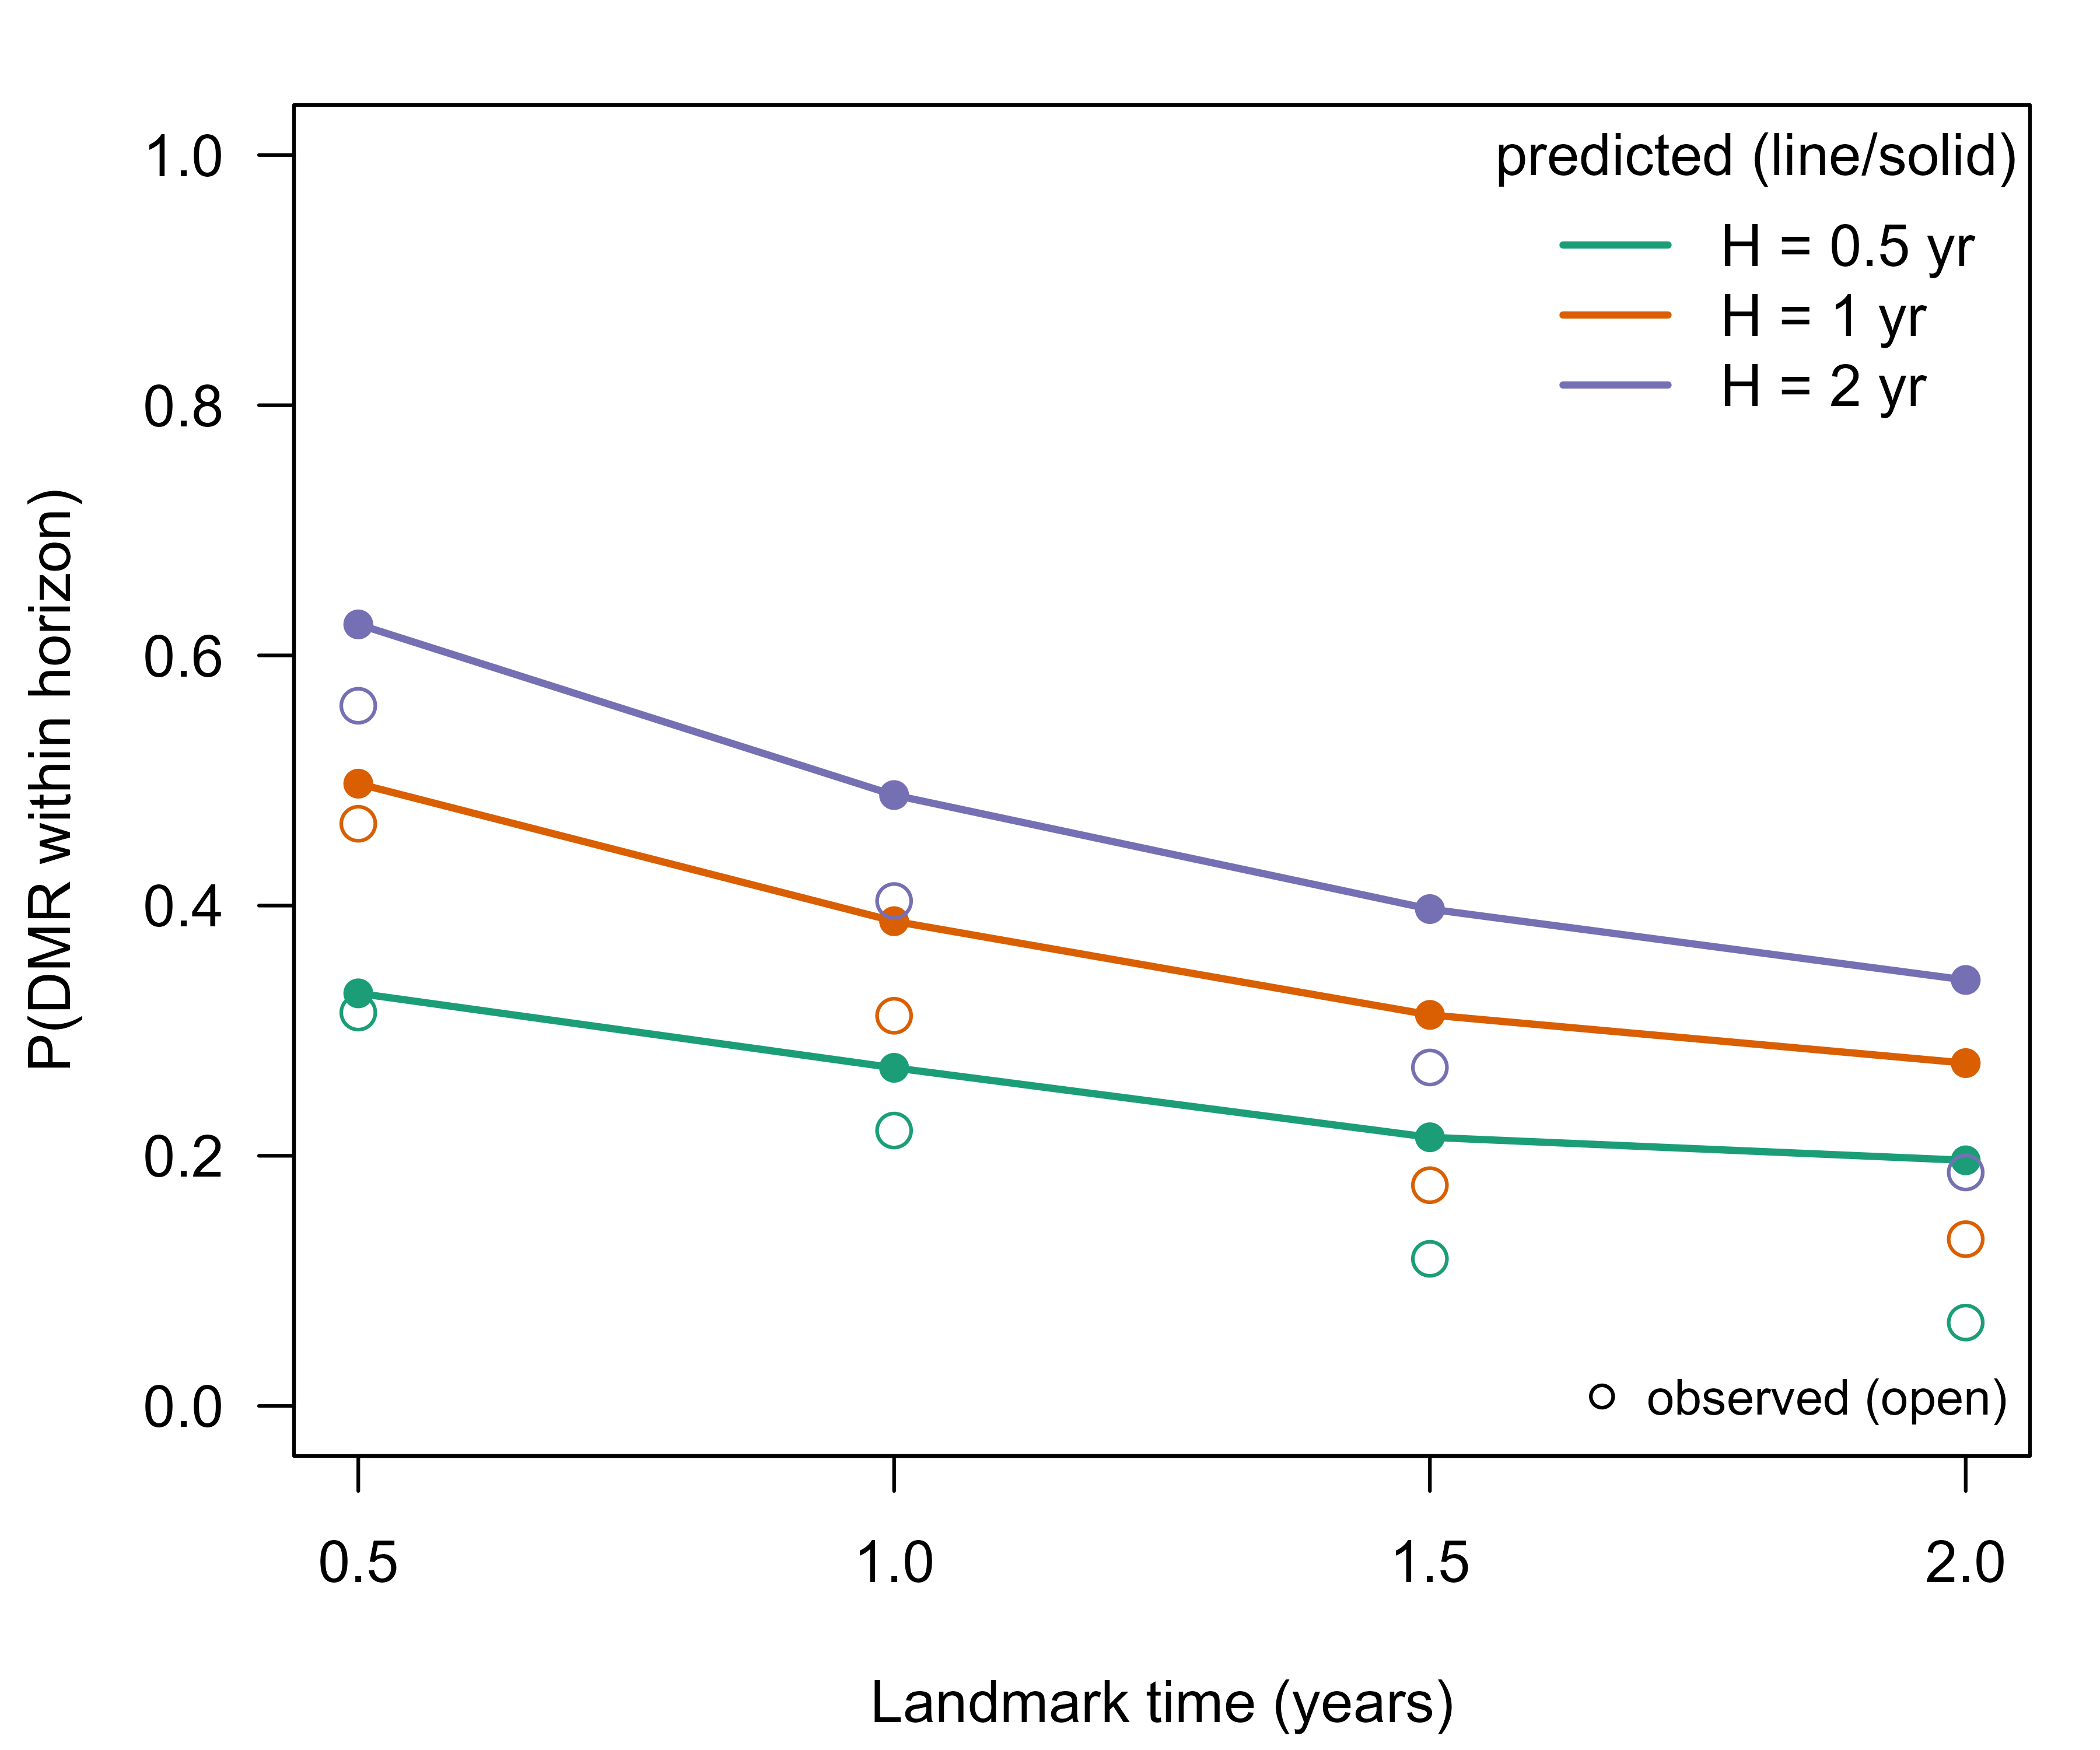
\includegraphics[width=0.7\linewidth]{figR_04_dynamic_prediction.png}
\caption{Predicted (solid) versus observed (open) within-horizon DMR
probability by landmark time, for horizons $H\in\{0.5,1,2\}$ years.}
\label{fig:dyn}
\end{figure}

\section{Summary}
On the simulated demonstration cohort both models recover the longitudinal
data-generating structure, the assay-floor model is well calibrated, and the
threshold-crossing formulation yields interpretable, well-calibrated
patient-level and dynamic DMR predictions. The threshold model's divergent
transitions should be resolved (higher \texttt{adapt\_delta} or a
reparameterized threshold term) before confirmatory use, and absolute DMR
probabilities benefit from the horizon-specific recalibration layer. Replacing
the simulated cohort with the real monitoring data reproduces this report for
the applied analysis.

\end{document}
